\documentclass[a4paper,11pt]{kth-mag}
\usepackage[T1]{fontenc}
\usepackage{textcomp}
\usepackage{lmodern}
\usepackage{amsmath}
\usepackage[swedish,english]{babel}
\usepackage{modifications}
\usepackage[usenames,dvipsnames,svgnames,table]{xcolor}
\usepackage[toc]{glossaries}
\usepackage{pgfplots}
\usepackage{graphicx}

\graphicspath{ {img/} }
\pgfplotsset{width=12cm,compat=1.9}

\newglossaryentry{computer}{
  name=computer,
  description=
  {is a programmable machine that receives input,
    stores and manipulates data, and provides
    output in a useful format}
}
\newglossaryentry{MLE}{
  name=Most Likelihood Estimate,
  description=
  {\todo yolo}
}


\newcommand{\todo}{ ... }

\newcommand{\numAnnotated}{12 }

\newcommand{\ngram}{$n$-gram\ignorespaces}
\newcommand{\ngrams}{$n$-grams\ignorespaces}

\newcommand{\category}{restaurant category }  % may become plural


\newif\ifhasStudiedFailures
\hasStudiedFailuresfalse

\newcommand{\loremipsum}{
  {\color{lightgray}
  Fruit two greater fifth over every. In female fourth good wherein herb
  Waters yielding itself. Female greater. Hath in, second appear tree in.
  Him, it seasons. Upon. Good you're. Winged green. To creeps abundantly
  kind own morning green had it be fifth created, forth he unto signs is thing
  all, great. Place night Gathering upon were forth light deep. Abundantly.
  Kind air beginning his void seed it dry. Own and spirit may dry abundantly
  beast good forth. The fifth beginning. Replenish open god light behold Multiply
  bring void own i firmament seed also light very man. \gls{computer}

  }
}

\makeglossaries

\title{Something, something, something, thesis...}

\subtitle{Getting a degree is hard}
\foreigntitle{Getting a degree is hard in swedish too}
\author{Mattis Kancans Envall}
\date{June 2016}
\blurb{Master's Thesis at CSC\\Supervisor: Johan Boye\\Examiner: Viggo Kann}
\trita{TRITA xxx yyyy-nn}


\begin{document}
\frontmatter
\pagestyle{empty}
\removepagenumbers
\maketitle
\selectlanguage{english}
\begin{abstract}
  This is a skeleton for KTH theses. More documentation
  regarding the KTH thesis class file can be found in
  the package documentation.

\loremipsum

\end{abstract}
\clearpage
\begin{foreignabstract}{swedish}
  Denna fil ger ett avhandlingsskelett.
  Mer information om \LaTeX-mallen finns i
  dokumentationen till paketet.

\loremipsum

\end{foreignabstract}
\clearpage
\tableofcontents*

\glsaddall
\printglossaries

\mainmatter
\pagestyle{newchap}
\part{Introduction}
\chapter{Introduction}
With increased internet usage, reviews online are becoming one of the most important resources when comparing businesses, services and products.
The increasing quantity of content makes for more reliable conclusions as more opinions can be taken into account, but it also poses a problem,
since there is a limit to what human readers can process.

Computers are obviously faster and more capable to handle big quantities of data, which suggests potential for using computers as aid when
interpreting review-like content. This is studied under the name \emph{Sentiment Analysis}, and has been in very active research the last ten years
thanks to increases in available data and recent efforts to monetize it.

This degree project studies describes sentiment analysis with regard to mining and summarizing opinions in reviews, and provides a detailed study of one of the problems in this process.

%This general problem is called \emph{sentiment analysis}\cite{liu2012sentiment} and is widely considered a hard, non-trivial problem.
%sentiment analysis is one of the most active fiels of research in NLP.

%The general problem of using computers and Natural Language Processing(NLP)-techniques to study opinions in text s called \emph{sentiment analysis}, and is one of the most active fields of study in NLP.

%In fact, recent trends of monetizing online content, not to mention the benefit of being able to

\section{Sentiment analysis}
Sentiment analysis\cite{liu2012sentiment} is the general task of from raw text extracting and interpreting expressions with associated sentiments. This involves classifying orientation (and possibly intensity) of found sentiments, and identifying what entity, and possibly what aspect of that entity, is subject to the expressed sentiments.

\subsection{Levels of sentiment analysis}
In general, sentiment analysis has been studied at three levels:

On the \emph{document level}, one overall sentiment of an entire document is identified. This is generally of limited use, as in most contexts, documents hold many opinions. Therefore most studies at the document level in some way handle conflicting opinions, although this may be done implicitly\cite[Chapter~3]{liu2012sentiment}. In document level sentiment analysis, the problem definition itself requires generalizations, which may invite to inaccurate over-simplifications.

\emph{Sentence level} sentiment analysis mitigates this risk of generalization; sentences are generally smaller than documents and thus less likely to hold conflicting opinions, so assuming there is at most one sentiment has less impact on results --- but the problem itself is not addressed. As an example, the sentence \emph{``Although the service is terrible, I still like this restaurant''} is arguably overall positive, but simply deeming it so excludes information which reduces quality of results and makes them susceptible to systematic errors.

%todo examples in table?
Ideally two opinions should be identified in the above sentence, one about \emph{service} and one about the reviewed entity in general. Sentiment analysis this fine grained is on the \emph{aspect level}. The goal is to find and classify individual opinions, which may  dealing with things like surjective opinions \emph{``food, service and ambiance were all great''}, conjunctions \emph{``tasty but expensive''}, implicit references \emph{``Easy to fit in my pocket''} really implies \emph{``good size''}, and implicit references \emph{``I had pasta. It was great''}'. As such, sentiment analysis on the aspect level is commonly referred to as the most complicated, as it consists of several sub-problems\cite[chapter 1]{liu2012sentiment}.


\subsection{Sentiment Classification}
Sentiment classification can be either a classification problem or regression analysis problem\cite{liu2012sentiment}, depending on whether results are expected to be discrete class-labels or a continuous measure of positively. In this report the discrete classification definition will be used unless otherwise specified.

Various approaches to sentiment classification exist, where approaches can generally be categorized as either grammatical\cite{todo}, statistical\cite{todo}, or a combination of the two.

The following subsections apply to text classification in general, and thus also to sentiment classification.

\section{WordNet and word relations}
\subsection{Word senses encapsulate meaning}
A few terms in linguistics are rather ambiguous and require definitions of usage. In this report it is used synonymously with the term \emph{lemma}, as defined by D. Jurafsky and J.H. Martin\cite{nlpbook}. Similarly, the definition of \emph{word sense} from the same source will be used to reference single meaning of a word; e.g. \textbf{bank$^1$} (``financial institution'') and \textbf{bank$^2$} (``sloping mound'') are different \emph{word senses} even though they share one \emph{word form}.

\subsection{\ngram modeling}
\ngram modeling is a versatile and widely used method of modeling languages. Typically the model consists of, for some $n$, all $n$-length sub-sequences of a longer sequence (i.e. one or many documents). Each unique sub-sequence is then referred to as a \ngram, and \ngrams of length \emph{1,2,3} are referred to as \emph{unigrams, bigrams} and \emph{trigrams}, respectively\cite{ngram}.

Typically counts or frequencies of individual \ngrams are used in tasks.

As an example, the \emph{bigrams} for the sentence \emph{``Languages are fun''} are:
\begin{quote}
  \vspace*{0.1cm}
  \centering
\emph{``\$ Languages''}, \emph{``Languages are''}, \emph{``are fun''}, \emph{``fun \$''},
\end{quote}
where \emph{\$} is a token meaning the start/end of sentence.

Although \ngram modeling can be applied to virtually any kind of sequence, this report henceforth will refer exclusively to \ngrams consisting of words.

If the probability of a word's occurrence in a sentence is known, then the probability of a sentence can be modeled using a \emph{unigram} model the following way thanks to the chain rule:
$$P(s) = \prod_{w_i \in s}P(w_i)$$, where $w_i$ is the $i$th word in the sentence, and $P$ is the probability of that word (usually basic )

Based on the Markov assumption, that the probability of a word's occurrence only depend on previous word in the sentence, the above can be extended to \emph{bigrams}:

$$\sum_{w_i}P(w_i|w_{i-1})$$

\subsection{Smoothing}
A general problem when statistically modeling based on existing data, is how the model should handle previously unseen entities. A naive \gls{MLE} would per definition assign a zero probability, since unseen would imply impossible. Since human language is virtually infinite even the reasonable sentences are innumerable, which means that no training data


\subsection{Back-off}

\subsection{Yelp's sentiment analyzer}

\subsection{Bias in data}
\label{subsec:bias}

\chapter{Methodology}
\section{Evaluation}
A common way to evaluate information retrieval tasks is \emph{precision} and \emph{recall}. Together they evaluate a systems quality, by evaluating the capacity to exclude irrelevant results, and include relevant results, respectively.

\subsection{Precision}
Precision is a measure of what fraction of retrieved results are considered relevant, in this work this means \todo.

It is defined as following:
$$Precision = \frac{\text {true positives}}{\text{true positives} + \text{false positives}}$$
%From this definition it should be clear that precision can by excluding uncertain items from retrieved results.

\subsection{Recall}
Similarly, recall is the fraction of relevant results that are retrieved:
$$Recall = \frac{\text {true positives}}{\text{true positives} + \text{false negatives}}$$

The reader may note from these definitions that more hesitance when including results would mean fewer false positives, but more false negatives, which implies that higher precision can be achieved at the cost of lower recall.

\section{Aspect clustering}
\subsection{Using WordNet}
Based on the observation that there is usually some key words with lexicographical connection to the cluster, an alternative approach to traditional classification is proposed. This is motivated since classification models need complicated smoothing techniques and big training data sets to achieve good results.


\section{Experiment setup}
For these experiments, Yelp reviews from the \category were manually annotated in various ways.


\numAnnotated sentences were manually annotated on the sentence level and divided into three parts: Training, testing and evaluation. During development the first two parts of the data-set were made available, whereas the evaluation set of sentences was kept separately to ensure reliable results. To ensure impartialness of methods and increase reliability of results, the only output allowed from the evaluation data set was strictly restricted to summaries of results (i.e. no individual results were presented with their outcome)\ifhasStudiedFailures, except for when failing instances were explicitly studied after method development was finished\fi.

\subsection{Getting data}

\begin{figure}[h]
  \centering
  \fbox{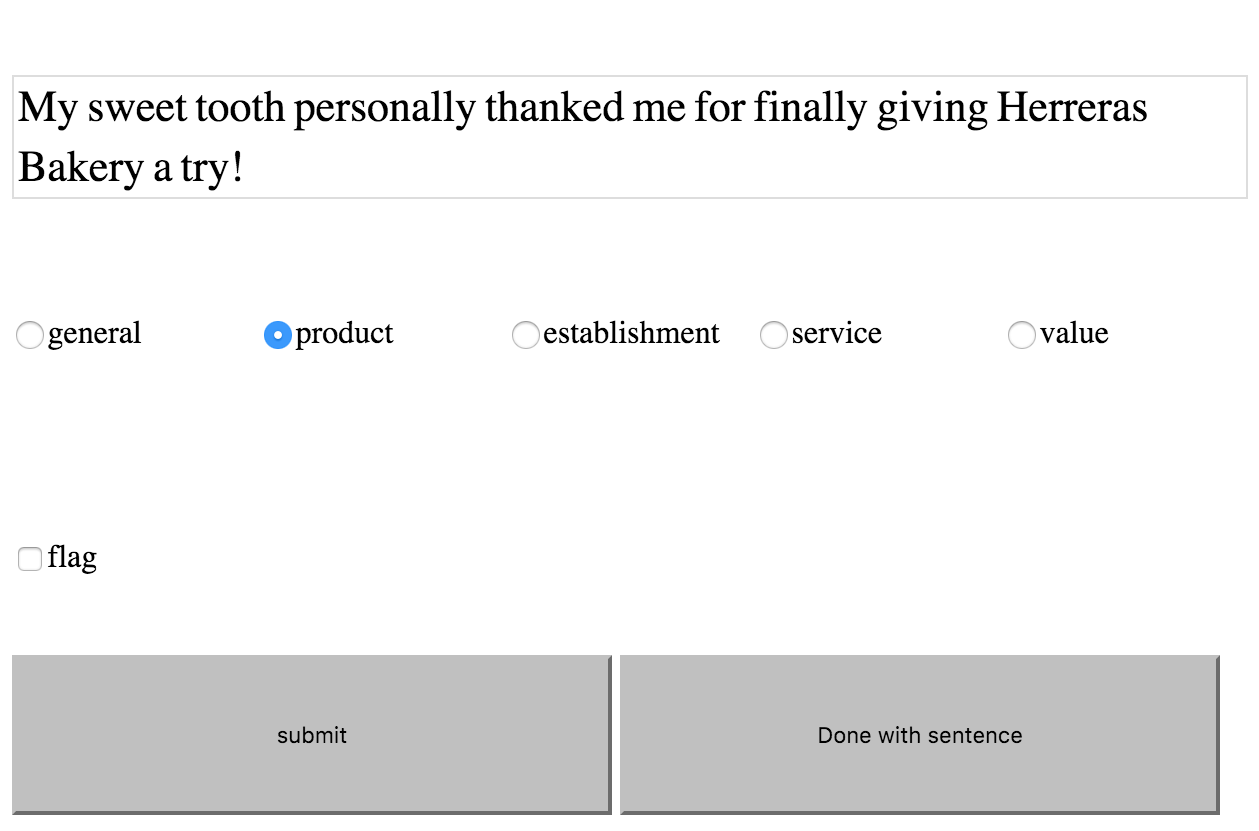
\includegraphics[width=12cm]{annontate_sentence.png}}
  \caption{Sentence annotations interface}
  \label{fig:annotate_sentence}
\end{figure}




% todo: annotations interface screenshot
% todo: num sentences table

% todo: accuracy / data size


\part{Results}


\begin{figure}[h]
  \centering

  \begin{tikzpicture}
    \begin{axis}[
        %title={Classifier performance based on data size},
        xlabel={Training data-set size},
        ylabel={Fraction of correctly classified},
        %xmin=0.3, xmax=0.7,
        %ymin=0.25, ymax=0.75,
        %xtick={0,20,40,60,80,100},
        %ytick={0,20,40,60,80,100,120},
        legend pos=north west,
        ymajorgrids=true,
        grid style=dashed,
      ]
      %\addplot table [x=n, y=p]{data/data_size_unigram.csv};
      \addplot table [x=n, y=p]{data/data_size_unigram_balanced.csv};
      \addplot table [x=n, y=p]{data/data_size_bigram.csv};
      \legend{
        %biased unigram,
        unigram,
        bigram
      }
    \end{axis}
  \end{tikzpicture}
  \caption{Sentence classification performance based on training data size}
  \label{fig:data_size}
\end{figure}

As expected, figure \ref {fig:data_size} shows that increased quantities of training data quickly yield improved results. This increment appears approximately linear, up to some point where it is expected to converge. Interesting is how the simpler unigram method quickly outperforms the bigram model, but that the bigram model sees more promising growth at the cut-off.




\begin{figure}[h]
  \centering
  \begin{tikzpicture}

  \begin{axis}[
      %title={Classifier performance per category},
      %xlabel={Categories},
      ylabel={Fraction of correctly classified},
      ybar, ymin=0,
      %bar width=20pt,
      xtick=data,
      x tick label style={rotate=45,anchor=east},
      xticklabels from table={data/per_category_unigram.csv}{n},
      xticklabel style={text height=1.5ex},
      ymajorgrids=true,
      grid style=dashed,
      legend pos=north east,
    ]
    \addplot table [x expr=\coordindex, y=p]{data/per_category_unigram.csv};
    \addplot table [x expr=\coordindex, y=p]{data/per_category_unigram_unbalanced.csv};
    \addplot table [x expr=\coordindex, y=p]{data/per_category_bigram.csv};
    \addplot table [x expr=\coordindex, y=p]{data/per_category_bigram_unbalanced.csv};
    \legend{unbalanced unigram, balanced unigram, balanced bigram, unbalanced bigram}
  \end{axis}
  \end{tikzpicture}
  \caption{Sentence classification performance per category}
  \label{fig:per_cat}
\end{figure}

\pagebreak
Section \ref{subsec:bias} introduced bias in data, along with some of its possible consequences. This motivates a more detailed study of classifier results on a per class basis. Figure \ref{fig:per_cat} shows some interesting properties.

First of all, comparison between the balanced/unbalanced versions of the classifier models show that, as expected, there seems to be bias towards the more frequent $product$-class and respectively against the infrequent $value$-class.

\loremipsum

\section{Preliminaries}
\bibliographystyle{plain}
\bibliography{references}

\end{document}
